\documentclass{article}

\usepackage{amsmath}
\usepackage{amsthm}
\usepackage{amsfonts}
\usepackage{thmtools}
\usepackage{stmaryrd}
\usepackage{natbib}
\usepackage{url}
\usepackage{array}
\usepackage{arydshln}
\usepackage{ifthen}
\usepackage{ifpdf}


\usepackage{tikz}
\usepackage{multirow}

\declaretheorem[numbered=yes,name=Lemma]{lemma}
\declaretheorem[numbered=yes,name=Definition]{definition}
\declaretheorem[numbered=yes,name=Specification]{specification}

\newcommand{\forcenewline}{$\phantom{v}$\\}

\newcommand{\update}[2]{[#1 \mapsto #2]}
\newcommand{\sem}[1]{\left\llbracket #1 \right\rrbracket}

%Math notation
\newcommand{\restrictfun}[1]{|_{#1}}
\newcommand{\parfun}{\rightharpoonup}
\newcommand{\monnefun}{\stackrel{\textit{\tiny{mon, ne}}}{\longrightarrow}}
\newcommand{\monfun}{\stackrel{\textit{\tiny{mon}}}{\longrightarrow}}
\newcommand{\defeq}{\stackrel{\textit{\tiny{def}}}{=}}
\newcommand{\nequal}[1][n]{\stackrel{\tiny{#1}}{=}}
\newcommand{\nsubeq}[1][n]{\stackrel{\tiny{#1}}{\subseteq}}
\newcommand{\nsupeq}[1][n]{\stackrel{\tiny{#1}}{\supseteq}}
\newcommand{\union}{\mathbin{\cup}}
\DeclareMathOperator{\dom}{dom}

\newcommand{\undefined}{\mathit{undefined}}

\newcommand{\false}{\mathit{false}}
\newcommand{\true}{\mathit{true}}

%Comments
\newcommand\lau[1]{{\color{purple} \sf \footnotesize {LS: #1}}}
\newcommand\dominique[1]{{\color{purple} \sf \footnotesize {DD: #1}}}

%Variables
\newcommand{\var}[1]{\mathit{#1}}
\newcommand{\hs}{\var{hs}}
\newcommand{\hv}{\var{hv}}
\newcommand{\rv}{\var{rv}}
\newcommand{\lv}{\var{lv}}
\newcommand{\pc}{\mathit{pc}}
\newcommand{\pcreg}{\mathrm{pc}}
\newcommand{\addr}{\var{a}}
\newcommand{\offset}{\var{offset}}
\newcommand{\word}{\var{w}}
\newcommand{\start}{\var{base}}
\newcommand{\addrend}{\var{end}}
\newcommand{\mem}{\var{mem}}
\newcommand{\reg}{\var{reg}}
\newcommand{\heapseg}{\var{hs}}
\newcommand{\heap}{\var{heap}}
\newcommand{\mode}{\var{mode}}
\newcommand{\perm}{\var{perm}}

\newcommand{\stdcap}[1][\perm]{\left(#1,\start,\addrend,\addr \right)}

%Memory projections
\newcommand{\plainproj}[1]{\mathrm{#1}}
\newcommand{\memheap}[1][\Phi]{#1.\plainproj{heap}}
\newcommand{\memreg}[1][\Phi]{#1.\plainproj{reg}}

\newcommand{\updateHeap}[3][\Phi]{#1\update{\plainproj{heap}.#2}{#3}}
\newcommand{\updateReg}[3][\Phi]{#1\update{\plainproj{reg}.#2}{#3}}

%Configuration end states
\newcommand{\failed}{\textsl{failed}}
\newcommand{\halted}{\textsl{halted}}

%Functions
\newcommand{\plainfun}[1]{\mathit{#1}}
\newcommand{\decode}{\plainfun{decode}}
\newcommand{\encode}{\plainfun{encode}}
\newcommand{\encodePerm}{\plainfun{encodePerm}}
\newcommand{\updatePcPerm}[1]{\plainfun{updatePcPerm}(#1)}

\newcommand{\executeAllowed}[1]{\plainfun{executeAllowed}(#1)}
\newcommand{\nonZero}[1]{\plainfun{nonZero}(#1)}
\newcommand{\readAllowed}[1]{\plainfun{readAllowed}(#1)}
\newcommand{\writeAllowed}[1]{\plainfun{writeAllowed}(#1)}
\newcommand{\withinBounds}[1]{\plainfun{withinBounds}(#1)}
\newcommand{\stdUpdatePc}[1]{\plainfun{updatePc(#1)}}

\newcommand{\readCond}[1]{\plainfun{readCondition}(#1)}
\newcommand{\writeCond}[1]{\plainfun{writeCondition}(#1)}
\newcommand{\execCond}[1]{\plainfun{executeCondition}(#1)}
\newcommand{\entryCond}[1]{\plainfun{entryCondition}(#1)}


%World operations
\newcommand{\future}{\mathbin{\sqsupseteq}}
\newcommand{\heapSat}[3][\heap]{#1 :_{#2} #3}

%Assembly labels
\newcommand{\codelabel}[1]{\mathit{#1}}
\newcommand{\init}{\codelabel{init}}
\newcommand{\malloc}{\codelabel{malloc}}
\newcommand{\counter}{\codelabel{counter}}
\newcommand{\iocap}{\codelabel{iocap}}

%Type(s)
\newcommand{\type}[1]{\mathrm{#1}}
\newcommand{\asmType}{\plaindom{AsmType}}


%Domains
\newcommand{\plaindom}[1]{\mathrm{#1}}
\newcommand{\Caps}{\plaindom{Cap}}
\newcommand{\Words}{\plaindom{Word}}
\newcommand{\Addrs}{\plaindom{Addr}}
\newcommand{\Mems}{\plaindom{Mem}}
\newcommand{\RegName}{\plaindom{RegisterName}}
\newcommand{\Regs}{\plaindom{Reg}}
\newcommand{\Heaps}{\plaindom{Heap}}
\newcommand{\HeapSegments}{\plaindom{HeapSegment}}
\newcommand{\Confs}{\plaindom{Conf}}
\newcommand{\Instrs}{\plaindom{Instructions}}
\newcommand{\nats}{\mathbb{N}}
\newcommand{\ints}{\mathbb{Z}}
\newcommand{\Perms}{\plaindom{Perm}}

\newcommand{\RegionName}{\plaindom{RegionName}}
\newcommand{\Worlds}{\plaindom{World}}
\newcommand{\StorePred}{\plaindom{StorePred}}
\newcommand{\UPred}[1]{\plaindom{UPred}(#1)}

%LR
\newcommand{\intr}[2]{\mathcal{#1}\sem{#2}}
\newcommand{\valueintr}[1]{\intr{V}{#1}}
\newcommand{\exprintr}[1]{\intr{E}{#1}}
\newcommand{\contintr}[1]{\intr{K}{#1}}
\newcommand{\regintr}[1]{\intr{R}{#1}}
\newcommand{\stdvr}{\valueintr{\asmType}}
\newcommand{\stder}{\exprintr{\asmType}}
\newcommand{\stdrr}{\regintr{\asmType}}
\newcommand{\stdkr}{\contintr{\asmType}}
\newcommand{\observations}{\mathcal{O}}
\newcommand{\npair}[2][n]{\left(#1,#2 \right)}

%Reference register/heap
\newcommand{\refreg}[1]{\lfloor #1 \rfloor}
\newcommand{\refheap}[1]{\langle #1 \rangle_h}

%Instructions
%No arguments
\newcommand{\fail}{\instr{fail}}
\newcommand{\halt}{\instr{halt}}
%One argument
\newcommand{\instr}[1]{\mathtt{#1}}
\newcommand{\oneinstr}[2]{\instr{#1} \; #2}
\newcommand{\jmp}[1]{\oneinstr{jmp}{#1}}
%Two arguments
\newcommand{\twoinstr}[3]{\instr{#1} \; #2 \; #3}
\newcommand{\jnz}[2]{\twoinstr{jnz}{#1}{#2}}
\newcommand{\isptr}[2]{\twoinstr{isptr}{#1}{#2}}
\newcommand{\setptr}[2]{\twoinstr{setptr}{#1}{#2}}
\newcommand{\move}[2]{\twoinstr{move}{#1}{#2}}
\newcommand{\store}[2]{\twoinstr{store}{#1}{#2}}
\newcommand{\load}[2]{\twoinstr{load}{#1}{#2}}
\newcommand{\lea}[2]{\twoinstr{lea}{#1}{#2}}
%Three arguments
\newcommand{\threeinstr}[4]{\instr{#1} \; #2 \; #3 \; #4}
\newcommand{\restrict}[3]{\threeinstr{restrict}{#1}{#2}{#3}}
\newcommand{\subseg}[3]{\threeinstr{subseg}{#1}{#2}{#3}}
\newcommand{\plus}[3]{\threeinstr{plus}{#1}{#2}{#3}}

%Permissions
\newcommand{\plainperm}[1]{\mathrm{#1}}
\newcommand{\noperm}{\plainperm{o}}
\newcommand{\readonly}{\plainperm{ro}}
\newcommand{\readwrite}{\plainperm{rw}}
\newcommand{\exec}{\plainperm{rx}}
\newcommand{\entry}{\plainperm{e}}
\newcommand{\rwx}{\plainperm{rwx}}

%OP sem
\newcommand{\diverge}[1][n]{\not\Downarrow_{#1}}
\newcommand{\step}[1][]{\rightarrow_{#1}}

\begin{document}
$\RegName$ contains $\pcreg$, but is otherwise some undefined, finite set.
\begin{align*}
\Addrs &::= \nats & & &
\Words &::= \Caps + \ints \\
\Regs  &::= \RegName \rightarrow \Words & & &
\Heaps &::= \Addrs \rightarrow \Words \\
\Perms &::= \{ \noperm, \readonly, \readwrite, \exec, \entry, \rwx\} & & &
\Mems  &::= \Regs \times \Heaps \\
\Caps  &::= \Perms \times \Addrs \times \Addrs \times \Addrs & & &
\Confs &::= \Mems + \{\failed, \halted \times \Mems\} \\
\HeapSegments &::= \Addrs \parfun \Words & & & &
\end{align*}

\begin{figure}[!h]
  \centering
  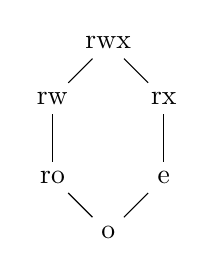
\begin{tikzpicture}[main node/.style={}]
  \node[main node] (1) {$\rwx$};
  \node[main node] (2) [below right of=1] {$\exec$};
  \node[main node] (3) [below of=2] {$\entry$};
  \node[main node] (4) [below left of=1] {$\readwrite$};
  \node[main node] (5) [below of=4] {$\readonly$};
  \node[main node] (6) [below right of=5] {$\noperm$};

  \path[every node/.style={font=\sffamily\small}]
    (1) edge (2)
    (2) edge (3)
    (3) edge (6)
    (1) edge (4)
    (4) edge (5)
    (5) edge (6);
\end{tikzpicture}
\caption{Permission hierarchy}
\label{fig:perm-hier}
\end{figure}
Notation:
$$\begin{array}{rcl}
i       &\in& \Instrs \\
r       &\in& \RegName\\
\mem    &::=& (\reg,\heap)\\
\pc     &\in& \Caps \\
\pcreg  &\in& \RegName \\
\Phi    &::=& \mem \in \Confs\\
\memheap&\in& \Heaps \\
\memreg &\in& \Regs \\
\addr   &\in& \Addrs\\
\perm   &\in& \Perms\\
(\perm,\start,\addrend,\addr) &\in& \Caps \\
n       &\in& \ints\\
\end{array}$$
Further definitions:
$$\begin{array}{rcl}
\lv    &::=& \refreg{r} \\
\hv    &::=& \refheap{r}\\
\rv    &::=& n \mid \lv \\
i      &::=& \fail \mid \halt \mid 
             \jmp{\lv} \mid \jnz{\lv}{\rv} \mid
             \isptr{\lv}{\rv} \mid \setptr{\lv}{\rv} \mid \\
       &   & \lea{\lv}{\rv} \mid\move{\lv}{\rv} \mid \load{\lv}{\hv} \mid \store{\hv}{\rv} \mid  \\
       &   & \restrict{\lv}{\rv}{\rv} \mid \subseg{\lv}{\rv}{\rv} \mid \plus{\lv}{\rv}{\rv}
\end{array}$$

\subsection*{Semantics}
Assume a $\decode$ function that decodes integer to instructions:
\begin{align*}
\decode &:\ints \rightarrow \Instrs
\end{align*}
Assume an $\encodePerm$ function that encodes a permission as an integer:
\begin{align*}
\encodePerm &: \Perms \rightarrow \ints
\end{align*}
\begin{align*}
  \Phi & \rightarrow \sem{\decode(\memreg(\pcreg))}(\Phi) & &                                   
                                                              \arraycolsep=0pt
                                                              \begin{array}{l}
                                                                \text{if $\memreg(\pcreg) = \stdcap$}\\
                                                                \quad\text{and $\start \leq \addr < \addrend$}\\
                                                                \quad\text{and $\perm \in \{ \exec,\rwx \}$ }
                                                              \end{array}\\
\Phi & \rightarrow \failed                                 & & \text{otherwise}
\end{align*}
It is assumed that address 0 is used for I/O, so whatever resides in location 0 after an execution can be seen as a result. As we will see in the semantics, it is assumed that the inital process starts with a readwrite capability for this location.
\begin{align*}
  \executeAllowed{\perm} &=
                           \begin{cases}
                             \true & \text{if } \perm \in \{ \rwx, \exec, \entry \} \\
                             \false & \text{otherwise}
                           \end{cases} \\
  \readAllowed{\perm} &=
                           \begin{cases}
                             \true & \text{if } \perm \in \{ \rwx, \exec, \readwrite, \readonly \} \\
                             \false & \text{otherwise}
                           \end{cases} \\
  \writeAllowed{\perm} &=
                           \begin{cases}
                             \true & \text{if } \perm \in \{ \rwx, \readwrite\} \\
                             \false & \text{otherwise}
                           \end{cases} \\
  \updatePcPerm{\perm,\start,\addrend,\addr} &=
                                     \begin{cases}
                                       (\perm,\start,\addrend,\addr) & \text{if $\perm\in\{ \rwx, \exec \}$} \\
                                       (\exec,\start,\addrend,\addr) & \text{if $\perm = \entry$}
                                     \end{cases} \\
  \nonZero{w} &=
                \begin{cases}
                  \true & \text{if $w\in \Caps$ or $w\in \ints$ and $w \neq 0$}\\
                  \false & \text{otherwise}
                \end{cases} \\
  \withinBounds{(\_,\start,\addrend,\addr)} &=
                                              \begin{cases}
                                                \true  & \text{if $\start \leq \addr \leq \addrend$} \\
                                                \false & \text{otherwise}
                                              \end{cases} \\
  \stdUpdatePc{\Phi} &=
                       \begin{cases}
                         \updateReg{\pcreg}{\var{newPc}} & 
                           \arraycolsep=0pt
                           \begin{array}{l}
                             \text{if $\memreg(\pcreg) = \stdcap$}\\
                             \quad\text{and $\var{newPc} = (\perm,\start,\addrend,\addr + 1)$}\\
                           \end{array} \\
                           \failed & \text{otherwise}
                       \end{cases} \\
\end{align*}
%TODO: \Phi.reg(rv) to some other notation. It should only look up reg, if it is a regname otherwise just the litteral.
\begin{align*}
  \sem{\fail}(\Phi)                        & = \failed \\
  \sem{\halt}(\Phi)                        & = (\halted,\Phi) \\
  \sem{\jmp{\lv}}(\Phi)                    & = 
                                             \begin{cases}
                                               \updateReg{\pcreg}{\updatePcPerm{c}} &
                                               \arraycolsep=0pt
                                               \begin{array}{l}
                                                 \text{if }\memreg(lv) = c \\
                                                 \quad\text{and }c=(\perm,\start,\addrend,\addr)\\
                                                 \quad\text{and }\executeAllowed{\perm}
                                               \end{array} \\
                                               \failed                              & \text{otherwise }
                                             \end{cases} \\
  \sem{\jnz{\lv}{\rv}}(\Phi)               & = 
                                             \begin{cases}
                                               \updateReg{\pcreg}{\updatePcPerm{\var{c}}} &
                                               \arraycolsep=0pt
                                               \begin{array}{l}
                                                 \text{if $\nonZero{\memreg(\rv)}$} \\ 
                                                 \quad\text{and $\memreg(lv) = c$} \\
                                                 \quad\text{and $c=(\perm,\start,\addrend,\addr)$}\\
                                                 \quad\text{and $\executeAllowed{\perm}$}
                                               \end{array}
                                               \\ %TODO Maybe combine with jump. (failed + this)
                                               \stdUpdatePc{\Phi} & \text{if not $\nonZero{\memreg(\rv)}$}\\
                                               \failed & \text{otherwise }
                                             \end{cases} \\
 \sem{\load{\refreg{r_1}}{\refheap{r_2}}}  & = 
                                             \begin{cases}
                                               \stdUpdatePc{\updateReg{r_1}{\var{w}}} &
                                               \arraycolsep=0pt
                                               \begin{array}{l}
                                                 \text{if } r_1 \neq \pcreg \\
                                                 \quad\text{and }\memreg(r_2) = (\perm,\start,\addrend,\addr) = \var{c} \\
                                                 \quad\text{and }\readAllowed{\perm} \text{ and } \withinBounds{\var{c}} \\
                                                 \quad\text{and }\var{w} = \memheap(\addr)
                                               \end{array}\\
                                               \failed & \text{otherwise }
                                             \end{cases}\\
 \sem{\store{\refheap{r_1}}{\refreg{r_2}}} & = 
                                             \begin{cases}
                                               \stdUpdatePc{\updateHeap{\addr}{\var{w}}} &
                                               \arraycolsep=0pt
                                               \begin{array}{l}
                                                 \text{if }\memreg(r_1) = (\perm,\start,\addrend,\addr) = \var{c} \\
                                                 \quad\text{and }\writeAllowed{\perm} \text{ and } \withinBounds{\var{c}} \\
                                                 \quad\text{and }\var{w} = \memreg(r_2)
                                               \end{array}\\
                                               \failed & \text{otherwise }
                                             \end{cases}\\
 \sem{\move{\refreg{r_1}}{\rv}}            & = \begin{cases}
                                                 \stdUpdatePc{\updateReg{r_1}{\memreg(\rv)}} & \text{if $r_1 \neq \pcreg$} \\ % For now we do this, so you need to use a jump to move stuff into pc.
                                                 \failed   & \text{otherwise }
                                 \end{cases}
\end{align*}
\begin{align*}
  \sem{\lea{\refreg{r_1}}{\rv}}            & =
                                             \begin{cases}
                                               \stdUpdatePc{\updateReg{r_1}{\var{c}}} &
                                                 \arraycolsep=0pt
                                                 \begin{array}{l}
                                                   \text{if either $n = \rv$ or $\rv = \refheap{r_2}$ and $n = \memreg(r_2)$} \\
                                                   \quad\text{and in either case $n \in \ints $} \\
                                                   \quad\text{and $\memreg(r_1) = \stdcap$}\\
                                                   \quad\text{and $\var{c} = (\perm,\start,\addrend,\addr + n)$}
                                                 \end{array}\\
                                               \failed               & \text{otherwise}
                                             \end{cases} 
\\ % In the M-Machine, lea checks whether the pointer stay within the allowed range in the pointer.
  \sem{\restrict{\refreg{r_1}}{\rv_1}{\rv_2}}           & =
                                             \begin{cases}
                                               \stdUpdatePc{\updateReg{r_1}{\var{c}}}  &
                                                 \arraycolsep=0pt
                                                 \begin{array}{l}
                                                   \text{if $r_1 \neq \pcreg$}\\
                                                   \quad\text{and $\memreg(\rv_1) = c'$}\\
                                                   \quad\text{and $c' = \stdcap$}\\
                                                   \quad\text{and either $\rv_2 = n$ or $\memreg(\rv_2) = n$}\\
                                                   \quad\text{and in either case $n \in \ints$}\\
                                                   \quad\text{and $\var{newPerm} = \encodePerm(n)$}\\
                                                   \quad\text{and $\var{newPerm} \sqsubseteq \perm$}\\
                                                   \quad\text{and $c = (\var{newPerm},\start,\addrend,\addr)$}
                                                 \end{array}\\
                                               \failed                   & \text{otherwise}
                                             \end{cases} \\ 
  \sem{\plus{\refreg{r_1}}{\rv_1}{\rv_2}}               & =
                                                          \begin{cases}
                                                            \stdUpdatePc{\updateReg{r_1}{n_1+n_2}} &
                                                            \arraycolsep=0pt
                                                            \begin{array}{l}
                                                              \text{if $r_1 \neq \pcreg$}\\
                                                              \quad\text{and $r_1\neq \pcreg$}\\
                                                              \quad\text{for $i \in \{1,2\}$}\\
                                                              \qquad\text{$n_i = \rv_i$ or $n_i = \memreg{\rv_i}$}\\
                                                              \qquad\text{and in either case $n_i \in \ints$}
                                                            \end{array}\\
                                                            \failed & \text{otherwise}
                                                          \end{cases}\\
  \sem{\isptr{\lv}{\rv}} & = \undefined \\ 
  \sem{\setptr{\lv}{\rv}} & = \undefined \\ 
  \sem{\subseg{\lv}{\rv}{\rv}} & = \undefined 
\end{align*}

\section{Examples}
\label{sec:examples}
\subsection{Ticket Dispenser}
\label{sec:tick-disp}
\newcommand{\size}{\var{size}}
\newcommand{\rio}{r_{io}}
\newcommand{\mrlen}{5cm}
\newcommand{\bracket}[1]{\multirow{#1}{*}{\ensuremath{
 \left . \vphantom{\begin{array}{l}
 \ifthenelse{\equal{#1}{1}}{3\\}{
    \ifthenelse{\equal{#1}{2}}{3\\3\\}{
    \ifthenelse{\equal{#1}{3}}{3\\3\\3\\}{
    \ifthenelse{\equal{#1}{4}}{3\\3\\3\\3\\}{
    \ifthenelse{\equal{#1}{5}}{3\\3\\3\\3\\3\\}{
    \ifthenelse{\equal{#1}{6}}{3\\3\\3\\3\\3\\3\\}{
      3\\3\\3\\3\\3\\3\\3\\ %7
  }}}}}}
  \end{array}} \right \}}}
}
\newcommand{\annotate}[2]{\multirow{#1}{\mrlen}{\scriptsize #2}}
Assume the instructions of some adversary resides in the memory starting at the memory location marked with $\codelabel{adv}$. Assume that the register $\rio$ initially contains a capability for the address in memory where I/O is written to (we assume this address is 0). We assume that entry capabilities for $\codelabel{adv}$ and $\malloc$ is ambiently available. The following is a test program for a ticket dispenser:
\[
  \begin{array}{r l l p{\mrlen}}
% Set io to -1
\init:     & \store{\refheap{\rio}}{-1} & \bracket{1} & \annotate{1}{Initialize io to $-1$} \\
% Store io capability just after jump to adv
           & \move{\refreg{r_0}}{\refreg{\pcreg}} & \bracket{3} & \annotate{3}{Store the io capability on the stack} \\
           & \lea{\refreg{r_0}}{\iocap} & & \\
           & \store{\refheap{r_0}}{\refreg{\rio}} & & \\
% Overwrite io register
           & \move{\refreg{\rio}}{0} & \bracket{1} & \annotate{1}{Overwrite io register} \\
% Allocate memory for ticket dispenser program
     & \move{\refreg{r_1}}{\size} &  \bracket{4} & \annotate{4}{Allocate memory for the ticket dispenser program (including memory for counter and capability for counter)}\\
           & \move{\refreg{r_0}}{\refreg{\pcreg}} & & \\
           & \lea{\refreg{r_0}}{3} & & \\
           & \jmp{\malloc} & & \\
% Save ticket dispenser code
           & \store{\refheap{r_1}}{(\encode(i_1))} & \bracket{7} & \annotate{7}{Store the ticket dispenser program in the newly allocated memory} \\
           & \lea{\refreg{r_1}}{1} & & \\
           & \store{\refheap{r_1}}{(\encode(i_2))} & & \\
           & \lea{\refreg{r_1}}{1} & & \\
           & \vdots & & \\
           & \store{\refheap{r_1}}{(\encode(i_7))} & & \\
           & \lea{\refreg{r_1}}{1} & & \\
% Save capability for counter
           & \move{\refreg{r_0}}{\refreg{r_1}} & \bracket{4} & \annotate{4}{Store a capability for the counter address after the ticket dispenser program} \\
           & \lea{\refreg{r_0}}{1} & & \\
           & \store{\refheap{r_1}}{\refreg{r_0}} & & \\
           & \lea{\refreg{r_1}}{1} & & \\
% Save capability for counter two addresses after jump to adv.
           & \move{\refreg{r_2}}{\refreg{\pcreg}} & \bracket{3} & \annotate{3}{Store a capability for the counter in this code} \\
           & \lea{\refreg{r_2}}{\counter} & & \\
           & \store{\refheap{r_2}}{r_0} & & \\
           & \move{\refreg{r_2}}{0} & \bracket{1} & \annotate{1}{Overwrite capability for counter} \\
% Save counter
           & \store{\refheap{r_1}}{0} & \bracket{1} & \annotate{1}{Initialize counter to 0} \\
% Change pointer to point to start of ticket dispenser code
           & \lea{\refreg{r_1}}{-8} & \bracket{1} & \annotate{1}{Capability points to start of td code \footnote{This is also the argument for the adversary}} \\
% Set up entry pointer to ticketDispenser for adv.
           & \restrict{\refreg{r_1}}{\refreg{r_1}}{(\encodePerm{(\entry)})} &\bracket{1} & \annotate{1}{Restrict cap. to td} \\
% Set up return pointer
           & \move{\refreg{r_0}}{\refreg{\pcreg}} & \bracket{3} & \annotate{3}{Setup a return pointer for the adversary} \\
           & \lea{\refreg{r_0}}{5} & & \\
           & \restrict{\refreg{r_0}}{\refreg{r_0}}{(\encodePerm{(\entry)})} & & \\
% jump to adv
           & \jmp{\codelabel{adv}} & \bracket{1} & \annotate{1}{Jump to the adversary} \\
           & 0 & \bracket{1} & \annotate{1}{Address reserved for io cap.} \\
           & 0 & \bracket{1} & \annotate{1}{Address reserved for counter cap.} \\
% retrieve io capability
           & \move{\refreg{r_0}}{\refreg{\pcreg}} & \bracket{3} & \annotate{3}{Retrieve the io capabiltiy} \\
           & \lea{r_0}{-2} & & \\
           & \load{\refreg{\rio}}{\refheap{r_0}} & & \\
% retieve counter capability
           & \lea{r_0}{1} & \bracket{2} & \annotate{2}{Retrieve the counter capability} \\
           & \load{\refreg{r_1}}{\refheap{r_0}} & & \\
% load the value of the counter
           & \load{\refreg{r_0}}{\refheap{r_1}} & \bracket{2} & \annotate{2}{Read the counter and write it to io address} \\
% store the value of the counter to io
           & \store{\refheap{\rio}}{\refreg{r_0}} & & \\
           & \halt
  \end{array}
\]
Here $\size$ is 9. The variables $\counter$ and $\iocap$ are resepctively the offsets to the addresses reserved for the counter and io capabilities. $i_1 \dots i_7$ refers to the instructions in the following ticket dispenser:
\[
  \begin{array}{r l}
    i_1 :& \move{\refreg{r_2}}{\refreg{\pcreg}} \\
    i_2 :& \load{\refreg{r_2}}{\size - 2} \\
    i_3 :& \load{\refreg{r_1}}{\refheap{r_2}}\\
    i_4 :& \plus{\refreg{r_3}}{\refreg{r_1}}{2} \\
    i_5 :& \store{\refheap{r_2}}{\refreg{r_3}} \\
    i_6 :& \move{\refreg{r_2}}{0} \\
    i_7 :& \jmp{\refreg{r_0}}
  \end{array}
\]
The heap layout for the above program can be seen in Figure~\ref{tab:tick-disp-heap}.
\begin{figure}[ht]
  \centering
  \begin{tabular}{ | c | l | }
    \hline
    Addr. & Content \\ \hline
    0   &  $i_1$ \\ \hline
    1   &  $i_2$ \\ \hline
    2   &  $i_3$ \\ \hline
    3   &  $i_4$ \\ \hline
    4   &  $i_5$ \\ \hline
    5   &  $i_6$ \\ \hline
    5   &  $i_7$ \\ \hline
    7   & Cap. for addr. 8 \\ \hline
    8   & The counter \\ \hline  
  \end{tabular}
  \caption{The heap layout for the ticket dispenser.}
  \label{tab:tick-disp-heap}
\end{figure}
In the JS paper, the ticket dispenser program dereferences the counter and returns the value. It does not seem like a similar thing would work here as the adversary can do even more. In particular, the adversary can execute a $\halt$ instruction that will cause the machine to halt (successfully). The adversary could also choose never to return to the return address, which we set up for him.
\begin{lemma}[Ticket dispenser test]
\label{lem:tckt-disp}
 Given a configuration $\Phi$, if
 \begin{description}
 \item[$\boldsymbol \memheap$] contains the ticket dispenser test program starting at the address labelled $\init$, 
 \item[$\boldsymbol \memheap$] contains the adversary code starting at label $\codelabel{adv}$. The adversary is assumed to have no capabilities on the heap, but it has access to the ambient $\malloc$ capability! \lau{maybe mention that malloc is also on the heap}
 \item[the heap segment $\boldsymbol{ \hs}$] contains all allocated addresses in the sense that any capability in $\Phi$ is a capability for a piece of memory in $\hs$,
 \item[$\boldsymbol{ \memreg(\pcreg)}$] is $(\rwx,\init,\init+\var{proglen}-1,\init)$, which is the only capability that grants any access to this part of the heap,
 \item[$\boldsymbol{ \memreg(\rio)}$] is $(\readwrite,0,0,0)$, which also is the only capability that grants access to this part of the heap, 
 \item[the remaining registers] all contains 0,
 \end{description}
 and $\Phi \rightarrow^* (\halted,\Phi')$, then the I/O address (that is $\memheap[\Phi'](0)$) contains either $-1$ or a number that is $\geq 0$ and even.
\end{lemma}
\lau{in the above lemma, what assumptions should we make on the adversary? In the js paper, we assume syntactically well-formed, do we here assume that the capability for the adversary is in the value relation? If so in what world should this be true? The one with just $\iota_{\var{adv},\var{adv end}}$?}
The variable $\var{proglen}$ is the length of the above program (which is about 57), so the in the initial configuration the $\pcreg$ register is assumed to have an execute and write permission for the area of the heap where the program resides.

The ticket dispenser test program uses $\malloc$. To be able to reason about programs that use $\malloc$, we assume that it obeys the following specification. If you provide it with one argument, namely the size of the allocation you wish and a return capability, then at some point $\pcreg$ will contain an executable capability based on this return capability and the return register will contain a $\rwx$ capability for the freshly allocated memory. 
\begin{specification}[Malloc]
Take $W_{\malloc}$ the world with exactly one island, namely the unspecified island $\iota_{\malloc}$ that governs the internal state of $\malloc$.  If we invoke $\malloc$ in a memory $h = \hs_{\var{frame}} \uplus \hs_{\var{footprint}}$ \\
\lau{Is $hs_{\var{frame}}$ supposed to be the rest of memory, so $h$ is something we can execute in? Is $\malloc$ allowed to allocate more memory, i.e., how does $\hs_{\var{footprint}}$ relate to $\hs_{\var{footprint}}'$?}\\
that is the disjoint sum of a frame part and a footprint part and the latter satisfies this world up to steps $n$, i.e., $\heapSat[\hs_{\var{footprint}}]{n}{W_{\malloc}}$. Then $\malloc$ will succesfully terminate and return a result in a heap $h' = \hs_{\var{frame}} \uplus \hs_{\var{footprint}}'$ that is the disjoint sum of the same unmodified frame part and a potentially new footprint part, such that there is a future world $W'$ of $W_{\malloc}$ consisting of exactly two islands, where the first is an instance of $\iota_{\malloc}$ and the second is the region $\iota_{\var{base},\var{end}}$\\
\lau{doesn't this invariant allow the newly allocated memory to contain capabilities?}\\
 for an appropriately-sized interval $\var{base},\var{end}$ and the new footprint part satisfies this new world $\heapSat[\hs_{\var{footprint}}']{?}{W'}$. 
\lau{at what step should this hold? Just some step $n'<n$?}\\
\lau{It should probably be more precise what it means to ``invoke'' $\malloc$ and for $\malloc$ to ``return'' something.}\\
\lau{How do we express that $\malloc$ can be ``trusted'' in the sense that it won't save the capab}
\end{specification}

\begin{proof}[Proof (Lemma~\ref{lem:tckt-disp})]
Let configuration $\Phi$ be given. Assume that the ticket dispenser test code resides in memory starting at address $\init$ along with the adversary code at address $\codelabel{adv}$. Also assume that capabilities for $\codelabel{adv}$ and $\malloc$ are ambiently available. Further assume that the register file contains the following:
\begin{enumerate}
\item $\memreg(\rio) = (\readwrite,0,0,0)$ 
\item $\memreg(\pcreg) = (\rwx,\init, \init + \var{proglen} - 1, \init)$
\item $\memreg(r) = 0$ for the remaining registers $r$ in the register file.
\end{enumerate}
Further assume $\Phi \rightarrow^* (\halted,\Phi')$. As the evaluation terminates, this must happen in a finite number of steps, say this number is $n$. We also assume that there is a heap segment $\hs$ as described in the lemma. If we execute $\Phi$ until just before the jump to $\malloc$, then a number of steps has occured, say $0<i<n$, further location 0 on the heap has been overwritten with $-1$, the io capability has been saved to the designated address on the heap, and the $\rio$ register has been overwritten with 0.

Now we need to jump to $\malloc$, so we need to make sure that the precondition in the specification is satisfied. To do this, we first need a world that models the part of the heap that is currently in use which is $\hs$. We pick the world $W$ to be:
\begin{align*}
  W(\codelabel{adv}) & = \iota_{\var{adv},\var{advend}} \\
  W(\init)           & = \iota_{\init,\init+\var{proglen} - 1} \\
  W(\rio)            & = \lambda W\ldotp \{(n,\hs) \mid \hs(0) = -1 \text{ or } \\
                     &   \hphantom{ = \lambda W\ldotp \{(n,\hs) \mid }\:\; \hs(0) \text{ even and positive} \}
\end{align*}
for all other addresses $a$ that are not captured in the above but are part of $hs$, we define a new region $r$ in $W$ where
\begin{align*}
  W(r) & = \iota_{a,a}
\end{align*}
Then we need to argue that $\heapSat[\hs]{n-i}{W}$. Given any address, in $\hs$ there is a region that covers that address, and the regions cover only the addresses in $\hs$. Now each of the heap segments have to be accepted by the respective regions. For the adversary, we assumed that it had no capabilities, so all the addresses contain intergers which i trivially in the value relation. The same goes for the heap segment with the ticket dispenser test program and the remaining addresses of the heap but addresses 0 \lau{need assumption about this.} The io address contains $-1$ at this point of the execution which mean that the heapsegment only consisting of address 0 is accepted in this world.

The remaining conditions in the specification are also satisfied, so there exists a configuration $\Phi'$
\end{proof}

\section{Logical Relation}
\label{sec:logical-relation}
\subsection{Worlds}
\[
  \StorePred = \Worlds \monnefun \UPred{\Addrs \parfun \Words}
\]
\[
\Worlds \cong \frac{1}{2} (\RegionName \parfun \StorePred)
\]

\[
  \iota_{\var{start},\var{end}} \; : \; \StorePred
\]
\begin{align*}
  \iota_{\var{start},\var{end}}(W) \defeq & \{ \npair{\heapseg} \mid \dom(\heapseg) = [\var{start},\var{end}] \land \\
                                     & \quad \forall \addr \in \dom(\heapseg) \ldotp \npair{\heapseg(\addr)} \in \stdvr(W) \}
\end{align*}

\begin{align*}
  \readCond{n,W,\start,\addrend} =        & \;\exists r \in \RegionName \ldotp \\
                                          & \;\quad \exists [\start',\addrend'] \supseteq [\start,\addrend] \ldotp W(r) \nsubeq[n-1] \iota_{\start',\addrend'} \\ & \\
  \writeCond{n,W,\start,\addrend} =       & \; \exists r \in \RegionName \ldotp \\
                                          & \;\quad \exists [\start',\addrend'] \supseteq [\start,\addrend] \ldotp W(r) \nequal[n-1] \iota_{\start',\addrend'} \\ & \\
  \execCond{n,W,\start,\addrend,\perm} =  & \; \forall n' < n \ldotp \forall W' \future W \ldotp \\
                                          & \; \quad \forall \addr \in [\start,\addrend] \ldotp \\
                                          & \; \qquad \npair[n']{(\perm,\start,\addrend,\addr)} \in \stder(W') \\ & \\
  \entryCond{n,W,\start,\addrend,\addr} = & \; \forall n' < n \ldotp \forall W' \future W \ldotp \\
                                          & \; \quad \npair[n']{(\rwx,\start,\addrend,\addr)} \in \stder(W') \\
\end{align*}

\[
\stdvr \; : \;  \Worlds \monfun \UPred{\Words}
\]
\begin{align*}
  \stdvr(W) \defeq & \{ \npair{i} \mid i \in \ints \} 
\union \\
                   & \{ \npair{\stdcap[\noperm] }  \} 
\union \\
                   & \{ \npair{\stdcap[\readonly] } \mid \readCond{n,W,\start,\addrend} \} \union \\
                   & \{ \npair{\stdcap[\readwrite] } \mid \writeCond{n,W,\start,\addrend} \} \union \\
                   & \{ \npair{\stdcap[\exec]} \mid \\
                   & \quad\readCond{n,W,\start,\addrend} \land \\
                   & \quad \execCond{n,W,\start,\addrend,\exec} \}
\union \\
% For the entry case a capability is acceptable, if we can change it to an execute permission and put it as the pc and we otherwise have valid words in the registers, then the register file should be valid.
                   & \{ \npair{\stdcap[\entry]} \mid \entryCond{n,W,\start,\addrend} \} \union \\
                   & \{ \npair{\stdcap[\rwx]} \mid \\
                   & \quad \writeCond{n,W,\start,\addrend} \land \\
                   & \quad \execCond{n,W,\start,\addrend,\exec} \land \\
                   & \quad \execCond{n,W,\start,\addrend,\rwx} \}
\end{align*}

Consider what the ``good observations'' should be? Before we do that - what should the end result of a computation be?
\begin{align*}
  \observations \quad : & \quad  \Worlds \monfun \UPred{\Confs} \\
  \observations (W) \defeq & \{ \npair{(\reg,\heap)} \mid \\
                           & \quad (\exists \reg', \heap' \ldotp (\reg,\heap) \step[n] (\reg',\heap')) \lor \\ %Define the step stuff 
                           & \quad (\exists \reg', \heap', i \leq n \ldotp (\reg,\heap) \step[i] \failed) \lor \\
                           & \quad (\forall \heap', i \leq n \ldotp (\reg,\heap) \step[i] (\halted,\heap')  \\
                           & \qquad \Rightarrow \npair[n-i]{\heap'(0)} \in \stdvr(W) \land \\
                           & \qquad \qquad \forall r \ldotp 0 \in \dom(W(r)) \ldotp \npair[n-i]{\heap' \restrictfun{\{0\}}} \in W(r)(W) )\}
\end{align*}
The ``good observations'' are as follows
\begin{itemize}
\item The execution does not stop in $n$ steps. 
\item The execution stops with a $\failed$.
\item The execution halts in at most $n$ steps with a valid value in in address 0 and the value at address 0 is also valid with respect to the world.
\end{itemize}
Address 0 is the designated I/O address.

Register-file relation:
\begin{align*}
  \stdrr \quad : & \quad \Worlds \monfun \UPred{\Regs} \\
  \stdrr(W) \defeq & \{ \npair{\reg} \mid \\
                    & \quad \forall r \in \RegName \setminus \{\pcreg\} \ldotp \\
                    & \qquad  \npair{\reg(r)} \in \stdvr(W) \}
\end{align*}

``Continuation'' relation:
\begin{align*}
  \stdkr \quad : & \quad  \Worlds \monfun \UPred{\Words} \\%TODO: What should this be?
  \stdkr(W) \defeq & \{ \npair{c} \mid \\
                   & \quad \forall v \in \stdvr(W)\ldotp \\
                   & \qquad  \forall W' \future W\ldotp %on the whiteboard, we had public future world.
                     \forall \heapSat{n'}{W'} \ldotp \forall \reg \in \stdrr(W') \\
                   & \qquad \quad (n,reg\update{r_0}{v}\update{\pcreg}{\updatePcPerm{c}}, \heap) \in \observations(W) \}
\end{align*}
\lau{$r_1$ contains the ``return value'', shouldn't that be the one we quantify over?} \\
\lau{When continuation is invoked, it has to be in registers, but here we do not require it to be in the value relation, so it seems impossible to show some of the required conditions.}
\dominique{$n'$ is unbound in the definition of $\stdkr$. }
\dominique{$v \in \stdvr(W)$ should be $v \in \stdvr(W')$ in the definition of $\stdkr$? }
\dominique{$\observations(W)$ should be $\observations(W')$ in the definition of $\stdkr$? }
``Expression'' relation:
\begin{align*}
  \stder \quad : & \quad \Worlds \monfun \UPred{\Words} \\%TODO: Check whether this needs to be monotone
  \stder(W) \defeq & \{ \npair{\pc} \mid \\
                   & \quad \forall \reg \in \stdrr(W) \ldotp \\
                   & \qquad \forall \npair{c} \in \stdkr(W) \ldotp \\
                   & \qquad \quad  \forall \heapSat{n}{W}, \heap_f \ldotp \\
                   & \qquad \qquad (n,\reg\update{r_0}{c}\update{\pcreg}{\pc},\heap \uplus \heap_f) \in \observations(W) \}
\end{align*}

\begin{definition}[Heap satisfaction/erasure]
\begin{align*}
  \heapSat{n}{W} & & \text{iff} & &
                                      \arraycolsep=0pt
                                      \begin{array}{l}
                                      \exists r: \dom(W) \rightarrow \HeapSegments \ldotp \\
                                      \qquad\heap = \biguplus_{\iota\in \dom(W)} r(\iota)\\
                                      \quad\text{and}\\
                                      \qquad\forall \iota \in \dom(W) \ldotp \npair{r(\iota)} \in W(\iota)(W)
                                      \end{array}\\
\end{align*}


\end{definition}
\begin{lemma}[Fundamental theorem of logical relations (FTLR)] \forcenewline
  For any $n \in \nats$, $W \in \Worlds$, and a word $\pc$, if  $\npair{\pc} \in \stdvr(W)$, then $\npair{\pc} \in \stder(W)$
\end{lemma}

\section{Related reading}
\label{sec:related-reading}

This is a list of related work that might be interesting to read in the context
of this project.

\subsection{Capability machines}
\label{sec:rw-cap-machines}

\subsubsection{M-Machine}
More than 20 years ago, \cite{Carter:1994:HSF:195473.195579} have described the
use of capabilities in the M-Machine. They do seem to have a reference for the
instruction set after all~\citep{Dally1997Memo59}; it seems like the server was
just temporarily down when we were looking for this the first time...

\subsubsection{CHERI}

The CHERI processor is a much more recent capability machine, described
by~\cite{Woodruff:2014:CCM:2665671.2665740,Watson2015Cheri}.

Another result of this project is also CheriBSD: an adaptation of FreeBSD to the
CHERI
processor.\footnote{\url{http://www.cl.cam.ac.uk/research/security/ctsrd/cheri/cheribsd.html}}
It is not separately described in a published paper, but mentioned in the papers
cited above and in some tech reports (see url). This work includes a
pure-capability ABI that could provide some interesting examples.

The CHERI team also has a webpage with all of their CHERI-related publications
(including TRs and
such)\footnote{\url{http://www.cl.cam.ac.uk/research/security/ctsrd/cheri/}}.

\subsection{Logical Relations}
\label{sec:rw-log-rel}

Some papers on logical relations that are relevant for this work are the
following:

\cite{Hur:2011:KLR:1926385.1926402} describe a logical relation between ML and
a (standard) assembly language for expressing compiler correctness.  Relevant
because they target an assembly language, and they use biorthogonality.

\cite{Dreyer:2010:IHS:1863543.1863566} describe a logical relation for a ML-like
language and use public/private transitions to reason about well-bracketed
control flow. Relevant because we are considering to cover an example of
enforcing well-bracketed control flow in a capability machine.

\cite{Devriese:2016ObjCap} describe a logical relation for a JavaScript-like
language with object capabilities.  Relevant because it treats object
capabilities, albeit in a JavaScript-like lambda calculus.

\bibliographystyle{plainnat}
\bibliography{refs}

\end{document}
